% % CVPR 2024 Paper Template; see https://github.com/cvpr-org/author-kit

% \documentclass[runningheads]{llncs}

% % ---------------------------------------------------------------
% % Include basic ECCV package
 
% % TODO REVIEW: Insert your submission number below by replacing '*****'
% % TODO FINAL: Comment out the following line for the camera-ready version
% % \usepackage[review,year=2024,ID=5548]{eccv}
% % TODO FINAL: Un-comment the following line for the camera-ready version
% \usepackage{eccv}

% % OPTIONAL: Un-comment the following line for a version which is easier to read
% % on small portrait-orientation screens (e.g., mobile phones, or beside other windows)
% %\usepackage[mobile]{eccv}


% % ---------------------------------------------------------------
% % Other packages

% % Commonly used abbreviations (\eg, \ie, \etc, \cf, \etal, etc.)
% \usepackage{eccvabbrv}

% % Include other packages here, before hyperref.
% \usepackage{graphicx}
% \usepackage{booktabs}

% \usepackage{multirow}
% \usepackage{makecell}
% \usepackage{wrapfig}
% \usepackage{xcolor} 
% \usepackage{pifont}
% % The "axessiblity" package can be found at: https://ctan.org/pkg/axessibility?lang=en
% \usepackage[accsupp]{axessibility}  % Improves PDF readability for those with disabilities.

% \usepackage{booktabs}
% \usepackage{multicol}
% \usepackage{colortbl}
% \usepackage{multirow}
% % \usepackage{amsthm}
% % \newtheorem{theorem}{Theorem} 
% % \newtheorem{lemma}{Lemma} 
% % \newtheorem{remark}{Remark}
% \usepackage{amssymb}
% \usepackage{pifont}
% \usepackage{comment}
% \usepackage[normalem]{ulem}
% \usepackage{xcolor}

% %%%%%%%%%%delete it before submission
% \newcommand{\wz}[1]{\textcolor{red}{\textit{Wenhui: #1}}}
% \newcommand{\pq}[1]{\textcolor{blue}{\textit{Peijie: #1}}}
% \newcommand{\xc}[1]{\textcolor{orange}{\textit{xiwen: #1}}}
% \newcommand{\ar}[1]{\textcolor{blue}{\textit{razi: #1}}}


% % It is strongly recommended to use hyperref, especially for the review version.
% % hyperref with option pagebackref eases the reviewers' job.
% % Please disable hyperref *only* if you encounter grave issues, 
% % e.g. with the file validation for the camera-ready version.
% %
% % If you comment hyperref and then uncomment it, you should delete *.aux before re-running LaTeX.
% % (Or just hit 'q' on the first LaTeX run, let it finish, and you should be clear).
% \definecolor{cvprblue}{rgb}{0.21,0.49,0.74}
% \usepackage[pagebackref,breaklinks,colorlinks,citecolor=cvprblue]{hyperref}

% %%%%%%%%% PAPER ID  - PLEASE UPDATE


% %%%%%%%%% TITLE - PLEASE UPDATE
% \title{{Supplementary Materials - DGR-MIL: Exploring Diverse Global Representation in Multiple Instance Learning for Whole Slide Image Classification}}

% %%%%%%%%% AUTHORS - PLEASE UPDATE
% \def\thefootnote{*}\footnotetext{These authors contributed equally to this paper.}
% \def\thefootnote{$\dagger$}\footnotetext{Corresponding author.}
% \author{Wenhui Zhu\inst{1* \dagger} \and
% Xiwen Chen\inst{2*} \and
% Peijie Qiu\inst{3*}  \and \\
% Aristeidis Sotiras\inst{3} \and Abolfazl Razi\inst{2} \and Yalin Wang\inst{1}
% }
% %
% \authorrunning{Zhu. Wenhui et al.}
% % First names are abbreviated in the running head.
% % If there are more than two authors, 'et al.' is used.
% %
% \institute{ Arizona State University, AZ, USA \\ {\tt\small \{wzhu59,ylwang\}@asu.edu} \and
% Clemson University, SC, USA \\ {\tt\small xiwenc@g.clemson.edu, arazi@clemson.edu} \and
% Washington University in St. Louis, MO, USA \\
% {\tt\small \{peijie.qiu,aristeidis.sotiras\}@wustl.edu }
% }
% \begin{document}
% \maketitle
% \appendix








\section{Measuring Diversity Based on Rate-distortion Theory}
\begin{figure*}[!ht]
    \centering
    \includegraphics[width=0.88\columnwidth]{Figure/diversity_vis.jpg}
    % \vspace{-0.4cm}
    \caption{(a) Examples of positive instances of with-bag and between-bag diversities measured by rate-distortion theory. (b) Histogram of the diversity measure within positive bags on the CAMELYON16 dataset. (c) The between-bag distinction measures the pair-wise similarity between bags.}  %The between-bag distinction measures the between-bag diversity among positive bags.
    \label{fig:1}
\end{figure*}
 Rate-distortion (RD) theory is a fundamental concept in \textit{information theory} to describe the lossy compression for arbitrary data sources with tolerable distortion. Here, rate $R$ refers to the number of bits or units per symbol of information required to represent the source data or signal; while distortion measures the quality of the reconstructed data compared to the original source data. 
 Mathematically, given an arbitrary source $X$, we can use finite bits $nR$ bits to encode a sequence of $n$ samples $X^n$ with $f_n(X^n)$ using a size codebook $2^{nR}$, and then decode it with
$\hat{X^n}=g_n(f_n(X^n))$. Accordingly, the reconstruction error for the sample sequence $x^n$ can be computed as $d(x^n,\hat{x}^n) := 1/n \sum_{i=1}^n d(x_i,\hat{x}_i)$ for some distance measure $d(\cdot)$. The most commonly used distortion metric is Mean Squared Errors (MSE), which is presented as $\epsilon^2:=1/n \sum_{i=1}^n (x_i-\hat{x}_i)^2$ and distortion $D$ is defined as $D:=\mathbb{E}[d(X^n, \hat{X}^n)]$ \cite{cover1999elements}. The rate $R$ is computed for a sequence with infinite length ($n \rightarrow \infty$) and distortion $D$. For a Gaussian source, given a finite dataset $\boldsymbol{X}=[\boldsymbol{x}_1,\boldsymbol{x}_2,\cdots,\boldsymbol{x}_n]\in \mathbb{R}^{d\times n}$, the theoretical coding rate with a small tolerable MSE distortion $\epsilon^2$, can be approximately estimated
as \cite{ma2007segmentation}, 
\begin{align}\label{eq:r0}
    R(\boldsymbol{X}, \epsilon) &:= \frac{1}{2} \log \operatorname{det}\left(\boldsymbol{I}+\frac{d}{n \epsilon^2} \boldsymbol{X} \boldsymbol{X}^{\top}\right),
\end{align}
where the unit of $ R(\boldsymbol{X}, \epsilon)$ is bit/dimension or nat/dimension for log base $2$ or $e$, respectively. Accordingly, the rate of the sub-space for each class $i$ can be approximated,
\begin{align}\label{eq:subclass}
       R^c_i(\boldsymbol{X}, \epsilon \mid{C}_i) :=\frac{1}{2} \log \operatorname{det}\left(\boldsymbol{I}+\frac{d}{|C_i| \epsilon^2} \boldsymbol{X}_{C_i} \boldsymbol{X}^{\top}_{C_i}\right) ,
\end{align}
% where $C_i\in\boldsymbol{C}$ is the index set of class $i$, $\boldsymbol{C}=C_1 \cup C_2 \cdots C_{c_T} $ is the set of all samples,
where $C_i$ is the index set of class $i$,
$c_T$ is the number of classes, $\boldsymbol{X}_{C_i}$ is a matrix using columns of $\boldsymbol{X}$ indexed by $C_i$ ($\boldsymbol{X}[:,C_i]$), and $|C_i|$ is the cardinality of $C_i$. 
Having adopted the assumption in \cite{yu2020learning}, we use the latent features extracted by the projector to estimate the diversity.

To better illustrate the way to compute the diversity, we copy Fig.\ref{fig:1} from the main body to here. In Fig.\ref{fig:1}.(b), we use Eq. \ref{eq:subclass} to compute the within-bag diversity, which refers to either all negative instances or positive instances (if applicable) from the same bag. The instances are treated as a data matrix $ \boldsymbol{X}$ in Eq.\ref{eq:r0}. We separately compute the diversity for each bag from the test set (80 negative bags and 49 positive bags), which results in a total of 129 negative within-bag diversity data points and 49 positive within-diversity data points. Then, we plot the histograms in Fig.\ref{fig:1}.(b), where the x-axis denotes the measure of diversity and the y-axis denotes the count (or frequency) of the diversity within the interval (i.g. the width and height in a bin, respectively).
It evidences both positive and negative within-bag instances are diverse and on a comparable scale. In Fig.\ref{fig:1}.(c), we use the rate reduction from \cite{yu2020learning} to compute the between-bag distinction of positive instances for every two bags. A rate reduction is presented as
\begin{align}
    \Delta R:=R(\boldsymbol{X}[:,C_1\cup C_2], \epsilon)- \sum_{i=1}^{2}\frac{|C_i|}{n} {R^c_i(\boldsymbol{X}, \epsilon \mid {C}_i)},
\end{align}
where $C_1$ and $ C_2$ are the index sets of two sub-space. This concept is used to describe the difference to encode the entire space and encode the sum of all sub-spaces, and a higher value indicates two sub-spaces are more discriminative; hence, we employed it as a metric to describe the distinction between two bags. In detail, we compare the distinction for every two positive bags. In each computation, 
$C_1$ and $ C_2$ denote the indices of positive instances from two different bags, respectively. $C_1\cup C_2$ denotes all instances from the selected two bags. Fig.\ref{fig:1}.(c) denotes the pair-wise distinction matrix, and we neglected the diagonal elements since they are zero. We also neglected the upper-triangle elements since this distinction matrix is symmetric.  
% It is noteworthy that rate reduction describe the difference to encode the entire space and encode the sum of all sub-spaces. Hence, it can be used to describe the distinction between two sub-spaces. 


\begin{table*}[t]
    \centering
    \caption{All training parameters setting for all methods in experiments. Here, Cosine annealing* denotes cosine decay with 20 epoch linear warmup from 1e-5. AMP represents automatic mixed precision, and the grad clip was clipped gradient norm constrained of model weight. Here, BCE was BCEWithLogitsLoss, which combines a sigmoid layer and the binary cross entropy loss.}
    \resizebox{0.99\textwidth}{!}{
    \begin{tabular}{l|l|l|l|l|l|l|l}\toprule
        \multicolumn{1}{c|}{\textbf{Parameters Setting}} & \textbf{AB-MIL} & \textbf{CLAM-SB/MB}& \textbf{DS-MIL}& \textbf{DTFD-MIL} & \textbf{Trans-MIL}  & \textbf{ILRA-MIL}  & \textbf{Our proposed Method }\\ \hline
        optimizer & Adam    &    Adam  &   Adam  &   Adam  &  Radam  & Adam & SGD   \\\cline{1-8}
        learning rate  &  1e-3    & 1e-4 &    1e-4  &   1e-4  &   2e-4  & 1e-4 & 5e-4   \\\cline{1-8}
        weight decay  &    0.005   & 1e-5 &   5e-3 &   1e-4 & 1e-5 & 1e-4 & 1e-4\\   \cline{1-8}                
        scheduler  &   Cosine  annealing* &  Cosine  annealing*& Cosine annealing &  MultiStepLR &   LookAhead~\cite{lookahead}  & Cosine annealing & Cosine annealing*\\ \cline{1-8}
        Dropout rate &           0.15    &           0.15 &   0.15  &   0.15 & 0.15  & 0.15  & 0.15    \\\cline{1-8}
        epoch  &  200  & 200  &   200 &   200    &   200  &   200 & 200 \\ \cline{1-8} 
        loss  &  BCE &  BCE &   BCE   &   BCE +  Tier-2 loss &  BCE   &  BCE   & $ \mathcal{L}_{ce} + \lambda_{tri} \mathcal{L}_{tri} + \lambda_{div}\mathcal{L}_{div}$\\ \cline{1-8}
        other settings  &  None  &  Early stop  &   Droppath = 0.2 &   grad clip = 5 & AMP & Xavier initialize & Warmup training strategy  \\ \cline{1-8} 
    \end{tabular}
    }
    \label{parameter}
    
\end{table*}



\section{Baseline Models Parameter Setting}
The baseline MIL methods include AB-MIL~\cite{ilse2018attention}, CLAM-SB, multi-attention CLAM-MB~\cite{clam-sb}, DS-MIL~\cite{li2021dual}, DTFD-MIL~\cite{zhang2022dtfd}, Trans-MIL~\cite{shao2021transmil} and ILRA-MIL~\cite{lowrankmil}. We follow the optimal parameter settings outlined in their original papers. The detailed parameters that we use to train all the baselines and the proposed model are shown in Table~\ref{parameter}. It is worth noting that our method adopts the linear learning rate warmup for the first 20 epochs, and details can be referred to~\ref{warmuptrainingstrategy}.

\subsection{ResNet-50 ImageNet Pre-Trained}
We use extracted features released by the DTFD-MIL. Each patch was embedded into a 1024-dimensional vector using a ResNet-18 pretrained on ImageNet~\cite{resnet}. The instance features are directly fed to MIL methods for training. In the experiments, we consistently set the middle layer (Some MIL methods including feed-forward layers before entering the aggregation method) output dimension to 512, For example, TransMIL~\cite{shao2021transmil},  ILRA~\cite{lowrankmil}, DTFD~\cite{zhang2022dtfd}, ABMIL~\cite{ilse2018attention}, and the proposed method.

\subsection{ResNet-18 ImageNet Pre-Trained}
\label{resnet18}
Different from DTFD-MIL, we employ the threshold filter method (entropy $<$ 5 discarded) to extract patches from raw WSIs~\cite{li2021dual}.  This results in fewer patches compared to DTFD-MIL. Each patch was embedded into a 512-dimensional vector as an instance feature. Here, we consistently set the middle layer output dimension to 256 in all MIL methods, including ILRA~\cite{lowrankmil}, DTFD~\cite{zhang2022dtfd}, ABMIL~\cite{ilse2018attention}, and the proposed method. Here, the TransMIL middle layers dimension output is 512, following the settings in its original paper~\cite{shao2021transmil}. Here, The TransMIL middle layers dimension output was 512, following the original paper setting~\cite{shao2021transmil}. The experiments section of the manuscript reveals a notable performance decline in most MIL methods. 

\subsection{Vision Transformer ImageNet Pre-Trained}
We employ the same threshold filter technique for patch extraction as we have done in the ResNet18 scheme. Each patch is transformed into a 768-dimensional vector using a vision transformer pre-trained on ImageNet. The middle layer output dimension in MIL methods with feed-forward layers, such as TransMIL~\cite{shao2021transmil}, ILRA~\cite{lowrankmil}, DTFD~\cite{zhang2022dtfd}, ABMIL~\cite{ilse2018attention}, and the proposed method, is set to 512. In line with the TransMIL study, the output dimension of its middle layers is also established at 512.

\subsection{Warm-up Training Strategy}
\label{warmuptrainingstrategy}
As outlined in our paper, a warm-up training strategy is incorporated in all experiments of the proposed method. This warm-up training can be described as follows:

\begin{equation}
    \mathcal{L}_{final} = \begin{cases} \mathcal{L}_{ce} , \ \text{iff} \ t < 20, \\ \mathcal{L}_{ce} + \lambda_{tri} \mathcal{L}_{tri} + \lambda_{div}\mathcal{L}_{div}, \ \text{iff} \ t > 20, \end{cases}
    \label{eqn:1}
\end{equation}
where t is the current epoch. The total training epoch is set to 200  for all experiments in this paper. We only employ the cross entropy classification loss to train our model at the first 20 epochs; while adding all the other losses for the latter epochs. The rationale behind this is that the randomly initialized global vectors usually lead to instability in training. The warmup training will help the global vectors to learn the meaningful instance relation in classification. This prevents poorly initialized global vectors from incorrectly misleading the modeling of instance correlations at the start.

\begin{table*}[t]
\centering
\caption{Comparision over efficiency among different transformer-based MIL aggregation methods in terms of the number of Parameters (M) and MACs (G) represent the model size and multiple-accumulated operation computational complexity, respectively.}
\label{computercomplexity}
\resizebox{0.5\columnwidth}{!}{
\begin{tabular}{l|cc}
\toprule %
     Models & Params(M) & MACs(G) \\
    \cmidrule(r){1-3}
    ILRA-MIL~\cite{lowrankmil}&  1.049  & 1.842\\
    Trans-MIL~\cite{shao2021transmil}& 3.040 & 2.409\\
    Our & 0.642 & 1.054\\

\bottomrule
\end{tabular}
}
\end{table*} 



\section{Efficiency Comparision of Transformer-Based MIL Aggregation Methods}
Take feature vectors extracted by ResNet-18 as an example, we apply the same hidden parameters as reported in the experiments. As shown in Table~\ref{computercomplexity}, the proposed method demonstrates superior efficiency compared to the other two transformer-based MIL aggregation methods, exhibiting notable advantages in terms of both model size and computational complexity. The cross-attention mechanism is more computationally efficient compared to the self-attention mechanism used across all instances. This efficiency stems from the use of an extremely short sequence of global vectors, which is substantially less in number than the total count of instances.

\noindent It is worth noting that ILRA-MIL~\cite{lowrankmil} employs self-attention for modeling the correlation between instances. Similarly, it also presents a larger number of parameters and is more computationally complex than the proposed method. The main reason is that they rewrite self-attention instead of self-attention with linear, and added the non-local pooling extra module. complexity~\cite{wang2020linformer,shen2021efficient,guo2022beyond}.

\section{Complexity of Diversity Loss}
The proposed diversity loss can be computed in a linear time complexity. 
For a global vector $\boldsymbol{G}\in \mathbb{R}^{K \times L}$, $\log\operatorname{det}(\boldsymbol{G}\boldsymbol{G}^T)=\sum_{i=1}^K\log(\lambda_i^2)$, where the main overhead is an SVD decomposition of $\boldsymbol{G}$ to get $\lambda_i$, resulting in a complexity of $\mathcal{O}(LK^2)\approx \mathcal{O}(L) $ due to $K$ is often set a small number (e.g., 5). 


\section{Statistical Test}
 We present the Wilcoxon signed-rank test and the critical difference diagram \cite{demvsar2006statistical} in Fig. \ref{fig:cd} with $\alpha=0.5$ significance level. Our method statistically outperforms all other competitors.


 \begin{figure}[h]
    \centering
    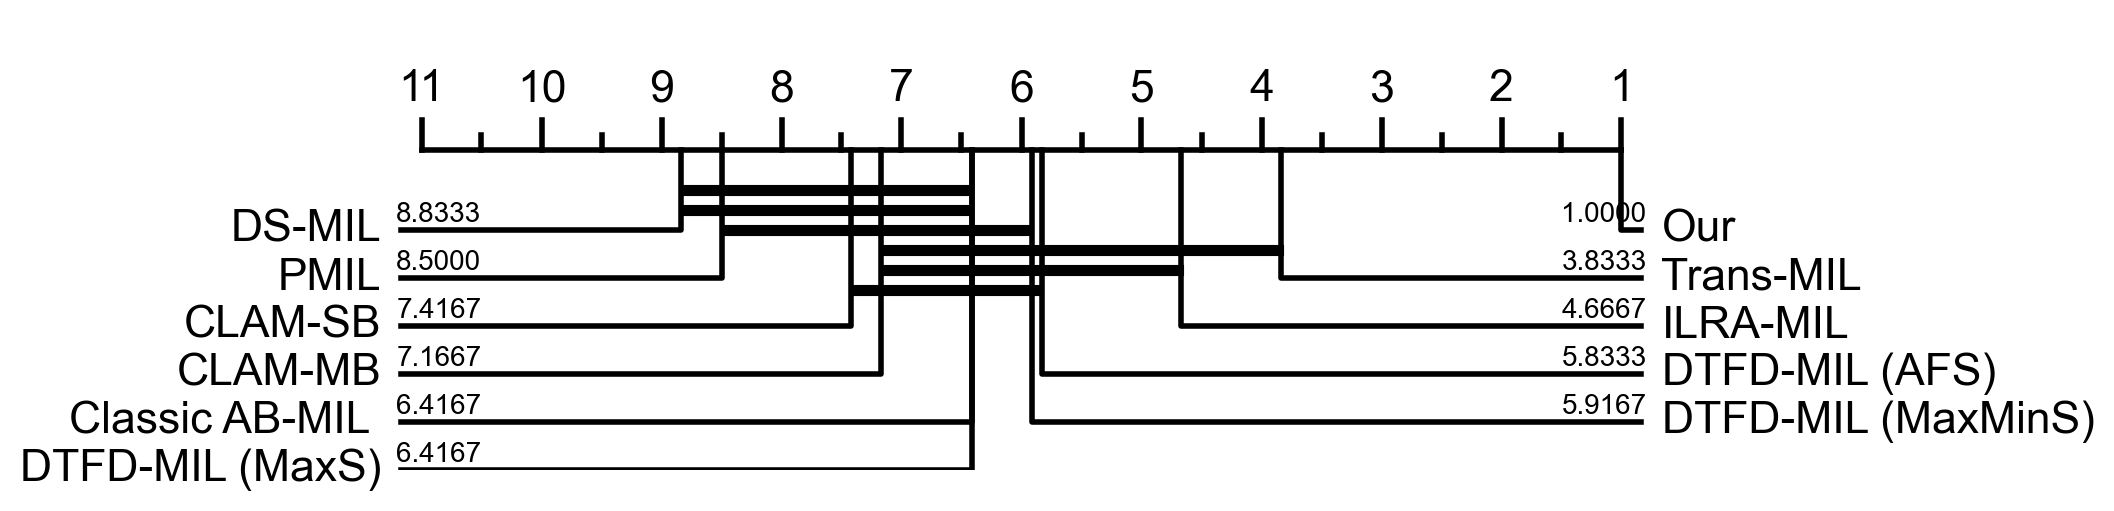
\includegraphics[width=0.7\columnwidth]{Figure/ranktest.png}
    \vspace{-0.3cm}
    \caption{Wilcoxon signed-rank test, average rank denoted by the number. No statistical difference found between methods connected with one thickness line in the critical difference diagram.
}
    \label{fig:cd}
    \vspace{-0.3cm}
\end{figure}


\section{Additional Results}
We present the additional experiments on CAMELYON16 with CTransPath feature extractor and classic MIL benchmarks. The results are shown in Table \ref{tab:ctrans} and Table \ref{tab:classic}, respectively.



\begin{table}[h]
% \vspace{-0.85cm}
\caption{Results on \textbf{CTransPath} extractor. We employ the 4-fold cross-validation using data split provided by DTFD.}
\label{tab:ctrans}
		\centering
		\resizebox{0.9\textwidth}{!}{
			\begin{tabular}{lccc}
				\toprule
                     & \multicolumn{3}{c}{CAMELYON16} \\
                      \cmidrule(r){2-4}
				  & Accuracy & F1 &  AUC  \\
				\midrule
				% & \multicolumn{3}{c}{\cellcolor{blue!20}\bf CTransPath as feature extractor } \\
                    Classic AB-MIL (\textit{ICML'18})   & $0.940_{(0.933,0.948)}$& $0.936_{(0.928,0.944)}$ & $0.951_{(0.932,0.970)}$\\ %
   
                    DS-MIL (\textit{CVPR'21})  &$0.929_{(0.898,0.959)}$  &$0.923_{(0.889,0.957)}$  &$0.942_{(0.916,0.968)}$  \\ %
                    
                    Trans-MIL (\textit{NeurIPS'21}) & $0.952_{(0.935,0.970)}$  & $0.949_{(0.930,0.968)}$  & $0.973_{(0.958,0.987)}$ \\ %
                    

                    DTFD-MIL (MaxMinS) (\textit{CVPR'22})  &$0.949_{(0.931,0.953)}$ & $0.933_{(0.906,0.937)}$ & $0.985_{(0.976,0.994)}$ \\ %
                    DTFD-MIL (AFS) (\textit{CVPR'22})  & $0.942_{(0.931,0.953)}$ & $0.922_{(0.906,0.937)}$ & $0.982_{(0.969,0.995)}$
                    \\%
                    ILRA-MIL (\textit{ICLR'23}) 
                    &$0.940_{(0.924,0.957)}$& $0.937_{(0.922,0.953)}$ & $0.961_{(0.946,0.975)}$ 
                      \\                 
                     \rowcolor{blue!8} 
                     % \rowcolor{yellow!18} 
                     \textbf{Our}  
%                      &$0.917
% _{(0.902
% ,0.931)}$& $0.913_{(0.898,0.928)}$ & $0.957_{(0.951,0.963)} $ & $0.908_{0.015}$ &$0.911_{0.018}$ &$0.963_{0.008}$  
&$\mathbf{0.972}_{(0.965, 0.979)}$& $\mathbf{0.971}_{(0.963, 0.978)}$ & $\mathbf{0.994}_{(0.991, 0.996)}$ \\ 
				\bottomrule
 			\end{tabular}}
    \vspace{-0.2cm}
\end{table}


\begin{table}[h]
  % \vspace{-0.6cm}
  \caption{Results on MIL benchmarks.}%The results of baselines are reported by DSMIL.
  % \vspace{-0.25cm}
  \centering
  \resizebox{0.9\textwidth}{!}{
  \begin{tabular}{l|ccccc}
    \toprule
    Methods     & MUSK1  & MUSK2 & FOX & TIGER & ELEPHANT \\
    \hline
     mi-Net & 0.889 $\pm$ 0.039  & 0.858 $\pm$ 0.049 & 0.613 $\pm$ 0.035 &  0.824 $\pm$ 0.034 &  0.858 $\pm$ 0.037   \\
    MI-Net &  0.887 $\pm$ 0.041 & 0.859 $\pm$ 0.046 & 0.622 $\pm$ 0.038 & 0.830 $\pm$ 0.032 & 0.862 $\pm$ 0.034       \\
    MI-Net with DS & 0.894 $\pm$ 0.042 & 0.874 $\pm$ 0.043 & 0.630 $\pm$ 0.037 & 0.845 $\pm$ 0.039 & 0.872 $\pm$ 0.032    \\
    MI-Net with RC & 0.898 $\pm$ 0.043 & 0.873 $\pm$ 0.044 & 0.619 $\pm$ 0.047 & 0.836 $\pm$ 0.037 & 0.857 $\pm$ 0.040    \\
    ABMIL &  0.892 $\pm$ 0.040 & 0.858 $\pm$ 0.048 & 0.615 $\pm$ 0.043 & 0.839 $\pm$ 0.022 & 0.868 $\pm$ 0.022   \\
    ABMIL-Gated & 0.900 $\pm$ 0.050 & 0.863 $\pm$ 0.042 & 0.603 $\pm$ 0.029 & 0.845 $\pm$ 0.018 & 0.857 $\pm$ 0.027   \\
    DP-MINN  & 0.907 $\pm$ 0.036 & 0.926 $\pm$ 0.043 & 0.655 $\pm$ 0.052 & 0.897 $\pm$ 0.028 & 0.894 $\pm$ 0.030  \\
    NLMIL & 0.921 $\pm$ 0.017 & 0.910 $\pm$ 0.009 & 0.703 $\pm$ 0.035 & 0.857 $\pm$ 0.013 & 0.876 $\pm$ 0.011 \\
    ANLMIL & 0.912 $\pm$ 0.009 & 0.822 $\pm$ 0.084 & 0.643 $\pm$ 0.012 & 0.733 $\pm$ 0.068 & 0.883 $\pm$ 0.014 \\
    DSMIL & 0.932 $\pm$ 0.023  & 0.930 $\pm$ 0.020 & 0.729 $\pm$ 0.018 & 0.869 $\pm$ 0.008 & 0.925 $\pm$ 0.007 \\
    \hline
    Our Method & \textbf{0.989 $\pm$ 0.033} & \textbf{0.970 $\pm$ 0.0458} & \textbf{0.785 $\pm$ 0.120} & \textbf{0.925 $\pm$ 0.055}  & \textbf{0.950 $\pm$ 0.044}   \\
    \bottomrule
  \end{tabular}
  }
  \label{tab:classic}
  \vspace{-0.25cm}
\end{table}

% \bibliographystyle{splncs04}
% \bibliography{ref}

% \end{document}